This chapter provides the necessary background on solar radiation in the Martian environment. \refSec{sec:MarsSolarEnergy:SolarRadiation} introduce variables and equations that must will be used when analyzing solar irradiance and insolation on Mars. Power and energy equations are presented in \refSec{sec:MarsSolarEnergy:PhotovoltaicEnergy}. \refSec{sec:MarsSolarEnergy:MissionSites} reviews the selected mission sites and presents their worst case daily insolations. The chapter is summarized and concluded in \refSec{sec:MarsSolarEnergy:SummaryAndConclusion}.

\section{Solar Radiation}
\label{sec:MarsSolarEnergy:SolarRadiation}
%\input{sections/mars-solar-energy/solar-radiation/references.tex}
\todo[inline]{\textbf{TODO:} Write section introduction.}

\subsection{Seasons}
\label{sec:MartianEnvironment:Seasons}
The red planet's axis is tilted away from the sun at \SI{25}{\degree}. Very much like Earth's \SI{23.5}{\degree} axial tilt, this results in seasons. Mars has an orbit with a semi-major axis of \SI{1.524}{\astronomicalunit} which translates to a Martian year corresponding to an orbital period of 687 days. Martian seasons are longer and for every Martian year 1.88 Earth years go by. Sidereal days are 24.62 hours long and solar days are 24.65 hours long. A Martian day, known as a Sol, is approximately 40 minutes longer than an Earth day. Mars' position on its orbit is described in terms of areocentric longitude of the Sun, $L_{s}$, and is measured Eastwards from $L_{s} = \SI{0}{\degree}$ at the northern hemisphere's Vernal equinox. The transition of Martian seasons are presented in Table \ref{tab:mars-seasonal-advances} with respect to areocentric longitudes.

\begin{table}[H]
  \centering
  \caption{Seasonal advances on Mars.}
  \label{tab:mars-seasonal-advances}
  \begin{tabular}{|l|l|l|}
  \hline
  \multirow{2}{*}{\textbf{\begin{tabular}[c]{@{}l@{}}Areocentric\\ Longitude\end{tabular}}} & \multicolumn{2}{c|}{\textbf{Seasonal Advance}} \\ \cline{2-3}
   & \multicolumn{1}{c|}{\textbf{Northern Hemisphere}} & \multicolumn{1}{c|}{\textbf{Southern Hemisphere}} \\ \hline
  \textbf{\si{0}{\degree}} & Vernal Equinox & Autumnal Equinox \\ \hline
  \textbf{\si{0}{\degree} to \si{90}{\degree}} & Spring & Autumn \\ \hline
  \textbf{\si{90}{\degree}} & Summer Solstice & Winter Solstice \\ \hline
  \textbf{\si{90}{\degree} to \si{180}{\degree}} & Summer & Winter \\ \hline
  \textbf{\si{180}{\degree}} & Autumnal Equinox & Vernal Equinox \\ \hline
  \textbf{\si{180}{\degree} to \si{270}{\degree}} & Autumn & Spring \\ \hline
  \textbf{\si{270}{\degree}} & Winter Solstice & Summer Solstice \\ \hline
  \textbf{\si{270}{\degree} to \si{360}{\degree}} & Winter & Summer \\ \hline
  \end{tabular}
\end{table}


\clearpage
\subsection{Dust}
\label{sec:MartianEnvironment:Dust}
The Martian surface is aeolianly active with varying concentration of airborn dust throughout the year due to processes of dust lifting, transportation, and deposition \citemarsenv{Kahre2006}.

\todo[inline]{\textbf{TODO:} Short overview of dust cycle on Mars.}
% See: https://www.nasa.gov/feature/goddard/2018/curiosity-photos-show-martian-dust-storm-growing

\subsubsection{Atmospheric Opacity}
\label{sec:MartianEnvironment:Dust:AtmosphericOpacity}
The density of suspended dust determines the atmospheric opacity, or optical depth, measured in $\tau$ factors. A $\tau$ factor between 0 and 0.5 indicates a clear to relatively clear day. Higher $\tau$ factors indicate dusty days with growing atmospheric dust opacity as represented in Figure \ref{fig:image:tau-factors} for simulated views pointing towards the Sun. \SI{99}{\percent} of sunlight is blocked at $\tau$ factor 4.7.

\todo[inline]{\textbf{TODO:} Source the 99\% claim.}

\begin{figure}[h]
  \centering
  \hypersetup{linkcolor=captionTextColor}
  \includegraphics[width=0.7\linewidth]{sections/mars-solar-energy/solar-radiation/images/tau-factors.png}\\
  \caption[Simulated views of atmospheric dust opacity for varying $\tau$ factors]
          {Simulated views of atmospheric dust opacity for varying $\tau$ factors. From left to right frames, tau factors of 1, 3, 5, 7, 9, and 11. Credits: NASA/JPL-Caltech/TAMU.}
  \label{fig:image:tau-factors}
\end{figure}

\subsubsection{Storms}
\label{sec:MartianEnvironment:Dust:Storms}

Dust storms are likely to occur while Mars approaches the Sun during the periphelion season between $L_{s} = \SI{185}{\degree}$ and $L_{s} = \SI{315}{\degree}$ \citemarsenv{Smith2019}. The Sun's proximity warms the atmosphere which creates temperature differences that produce dust lifting winds. The process is exacerbated by the release of carbon dioxide from the evaporating winter polar cap which thickens the atmosphere and increases surface pressure so that dust particles remain airborn. Figure \ref{fig:image:global-dust-storm-timing} shows the the timing of global dust storms until \ac{MY} 34.

\begin{figure}[h]
  \centering
  \hypersetup{linkcolor=captionTextColor}
  \includegraphics[width=0.4\linewidth]{sections/mars-solar-energy/solar-radiation/images/timin-of-observed-global-dust-storms.png}\\
  \caption[Timing of observed global dust storms on Mars]
          {Timing of observed global dust storms on Mars is concentrated in the season near the periphelion. Taken from \citemarsenv{Smith2019}.}
  \label{fig:image:global-dust-storm-timing}
\end{figure}

Global dust storms that cover an area of over \SI{e7}{\kilo\meter\squared} have a yearly probability of \SI{30}{\percent} to \SI{80}{\percent} whereas local dust storms that cover an area less than \SI{e7}{\kilo\meter\squared} occur with a \SI{5}{\percent} probability \citepower{Kerslake1999}. Local dust storms typically have a $\tau$ factor of approximately 1 \citepower{Kerslake1999} whereas the largest in situ $\tau$ factor recorded by \ac{MER} Opportunity was 10.8 in \ac{MY}34 near $L_{s} = \SI{180}{\degree}$.


\subsection{Solar Radiation}
\label{sec:MartianEnvironment:SolarRadiation}

\todo[inline]{\textbf{TODO:} Short introduction on Solar Radiation.}

The radiation profiles illustrated in this section with respect to Martian surface are for MER Opportunity's final location at Endeavour Crater. Calculations presented in this section as well their nomenclatures are taken from \citemarsenv{Appelbaum1989}, \citemarsenv{Appelbaum1990}, \citemarsenv{Appelbaum1991}, \citemarsenv{Appelbaum1993}, and \citemarsenv{Appelbaum1994} where profiles at locations of \ac{VL1} and \ac{VL2} can be observed.

\subsubsection{Irradiance}
\label{sec:MartianEnvironment:SolarRadiation:Irradiance}

Beam irradiance is the total solar flux density expressed in \si{Wm^{-2}}. It is a measure of solar radiation from direct sunlight. At the top of the Martian atmosphere the instantaneous beam irradiance, $G_{ob}$, is a function the areocentric longitude $L_{s}$:

\begin{equation}
  \label{eq:G_ob}
  G_{ob} = 590 \frac{[1 + e \cos{(Ls - 248)}]^2}{(1-e^2)^2}
\end{equation}

Where \SI{590}{Wm^{-2}} is the mean beam irradiance at the top of the Martian atmosphere, $L_{s} - \SI{248}{\degree}$ is the true anomaly, and $e$ is the Mars eccentricity. The variation of $G_{ob}$ is presented in Figure \ref{fig:plot:beam-irradiance-top-of-mars-atmosphere}. At its closest, the perihelion, Mars is at a distance of \SI{1.381}{\astronomicalunit} from the Sun with a beam irradiance on top of its atmosphere reaching its maximum of \SI{718}{Wm^{-2}} at $L_{s} = \SI{248}{\degree}$. At its furthest of \SI{1.666}{\astronomicalunit}, the aphelion, beam irradiance reaches its minimum of \SI{494}{Wm^{-2}} at $L_{s} = \SI{71}{\degree}$.

\begin{figure}[H]
  \centering
  \hypersetup{linkcolor=captionTextColor}
  \includegraphics[width=0.5\linewidth]{sections/mars-solar-energy/solar-radiation/plots/gob-daily-variations.png}\\
  \caption[Beam irradiance at top of Mars atmosphere as a function of Areocentric Longitude]
          {Beam irradiance at top of Mars atmosphere as a function of Areocentric Longitude}
  \label{fig:plot:beam-irradiance-top-of-mars-atmosphere}
\end{figure}

Further parameterization becomes necessary in order to measure beam irradiance on a horizontal surface at the top Mars atmosphere where the solar zenith angle $z$ must be considered. The solar zenith angle itself is a function of planetary latitude $\phi$, declination angle $\delta$, and hour angle $\omega$ measured from the true noon westward \citemarsenv{Appelbaum1990}. Expressed as $G_{obh}$, it is presented in Equation \ref{eq:G_obh}:

\begin{equation}
  \label{eq:G_obh}
  G_{obh} = G_{ob}\cos{z}
\end{equation}

where $z$ is given by:

\begin{equation}
  \label{eq:cosz}
  \cos{z} = \sin{\phi}\sin{\delta} + \cos{\phi}\cos{\delta}\cos{\omega}
\end{equation}

Solar radiation calculations using Equation \ref{eq:G_obh} as a function of Solar time are presented in Figure \ref{fig:plot:diurnal-variation-of-beam-irradiance-on-a-horizontal-surface-at-top-of-mars-atmosphere}.

\begin{figure}[h]
  \centering
  \hypersetup{linkcolor=captionTextColor}
  \includegraphics[width=0.5\linewidth]{sections/mars-solar-energy/solar-radiation/plots/gobh-diurnal-over-endaveaour-crater.png}\\
  \caption[Diurnal variation of beam irradiance on a horizontal surface at top of Mars atmosphere above Endaveaour Crater]
  {Diurnal variation of beam irradiance on a horizontal surface at top of Mars atmosphere above Endaveaour Crater.}
  \label{fig:plot:diurnal-variation-of-beam-irradiance-on-a-horizontal-surface-at-top-of-mars-atmosphere}
\end{figure}

Obtaining the irradiance on the surface of Mars requires the atmospheric opacity $\tau$ as an additional parameter. A distinction exists between global, direct, and diffuse beam irradiance where global beam irradiance $G_{h}$ is the sum of direct, $G_{bh}$, and diffuse beam irradiances, $G_{dh}$:

\todo[inline]{\textbf{TODO:} Explain scattering and diffuse irradiance.}

% TOOD: Mention scattering: https://ntrs.nasa.gov/archive/nasa/casi.ntrs.nasa.gov/20040191326.pdf

\begin{equation}
  \label{eq:G_h_1}
  G_{h} = G_{bh} + G_{dh}
\end{equation}

The expression for $G_{h}$ and $G_{bh}$ are presented in Equations \ref{eq:G_h} and \ref{eq:G_bh}:

\begin{equation}
  \label{eq:G_h_2}
  G_{h} = G_{ob}\cos{z}\frac{f(z,\tau)}{0.9}
\end{equation}

where $f(z,\tau)$ is the normalized net flux function derived from the net solar flux integrated over the solar spectrum on the Martian surface and 0.9 comes from the $(1-albedo)$ expression for an albedo of 0.1 \citemarsenv{Appelbaum1989}.

\begin{equation}
  \label{eq:G_bh}
  G_{bh} = G_{ob}\cos{z}\exp\left(\frac{-\tau}{cos{z}}\right)
\end{equation}

Diurnal irradiance profiles at Endaveour Crater are presented in Figure \ref{fig:plot:irradiances-phi} for different planetary latitudes during the perihelion. At $L_{s} = \SI{248}{\degree}$ the northern hemisphere is in mid-Autumn whereas the southern hemisphere in mid-Spring, as such irradiances are much larger at $\phi = \SI{-40}{\degree}$ and $\phi = \SI{-20}{\degree}$ than they are at $\phi = \SI{0}{\degree}$ and $\phi = \SI{40}{\degree}$.

\begin{figure}[h]
\captionsetup[subfigure]{justification=centering}
\vspace{-2ex}
	\centering
    %% setup sizes
    \setlength{\subfigureWidth}{0.50\textwidth}
    \setlength{\graphicsHeight}{80mm}
    %% kill hyper-link highlighting
    \hypersetup{hidelinks=true}%
    %% the figures
%% 1st row
  	\begin{subfigure}[t]{\subfigureWidth}
      \centering
  		\includegraphics[height=\graphicsHeight]{sections/mars-solar-energy/solar-radiation/plots/gh-gbh-gdh-variation-1-for-ls-248-phi-20-tau-05-and-albedo-027.png}
  		\subcaption{$\phi = \SI{-40}{\degree}$}
  		\label{fig:sub:irradiance-phi-m20}
  	\end{subfigure}\hfill
    \begin{subfigure}[t]{\subfigureWidth}
      \centering
  		\includegraphics[height=\graphicsHeight]{sections/mars-solar-energy/solar-radiation/plots/gh-gbh-gdh-variation-2-for-ls-248-phi-0-tau-05-and-albedo-027.png}
  		\subcaption{$\phi = \SI{-20}{\degree}$}
  		\label{fig:sub:irradiance-phi-0}
  	\end{subfigure}\\[0.8ex]
%% 2nd row
    \begin{subfigure}[t]{\subfigureWidth}
      \centering
  		\includegraphics[height=\graphicsHeight]{sections/mars-solar-energy/solar-radiation/plots/gh-gbh-gdh-variation-3-for-ls-248-phi-20-tau-05-and-albedo-027.png}
  		\subcaption{$\phi = \SI{0}{\degree}$}
  		\label{fig:sub:irradiance-phi-p20}
  	\end{subfigure}\hfill
	   \begin{subfigure}[t]{\subfigureWidth}
      \centering
  		\includegraphics[height=\graphicsHeight]{sections/mars-solar-energy/solar-radiation/plots/gh-gbh-gdh-variation-4-for-ls-248-phi-40-tau-05-and-albedo-027.png}
  		\subcaption{$\phi = \SI{20}{\degree}$}
  		\label{fig:sub:irradiance-phi-p40}
	   \end{subfigure}\hfill
	\caption{Diurnal variation of global, beam, and diffuse irradiance on Mars horizontal surface at different planetary latitudes.}
	\label{fig:plot:irradiances-phi}
\vspace{-2ex}
\end{figure}

\clearpage
\subsubsection{Insolation}
\label{sec:MartianEnvironment:SolarRadiation:Insolation}

Solar insolation is the amount solar radiation incident on a planetary surface during a time period. It is expressed in \si{Whm^{-2}} and obtained by integrating the equations of irradiance over a time period between $\omega_1$ and $\omega_2$. Thus, insolation on a horizontal surface at the top of Mars atmosphere, denoted as $I_{obh}$, is obtained by integrating Equation \ref{eq:G_h_2} of $G_{obh}$.

Global, beam, and diffuse insolations on a horizontal Mars surface are denoted as $I_{h}$, $I_{bh}$, and $I_{dh}$ respectively. Their values are obtained by integrating \ref{eq:G_h_2} for $I_{h}$ and \ref{eq:G_bh} for $I_{bh}$. Diffuse insolation $I_{dh}$ is obtained through the same relationship presented in Equation \ref{eq:G_h_1}. The variation of insolation as a function of $L_{s}$ for different levels of atmospheric opacities are illustrated in Figure \ref{fig:plot:insolation-ls}. Evidently, the insolation curves peak at the perihelion with $L_{s} = \SI{248}{\degree}$ and reach their lowest during the aphelion with $L_{s} = \SI{71}{\degree}$. Due to light scattering by airborn Martian dust \citemarsenv{Merikallio2013}, diffuse insolation is already the largest component contributing to the global insolation at $\tau = 1$. On a dusty day at $\tau = 3$, global insolation is mostly diffuse.

\begin{figure}[h]
\captionsetup[subfigure]{justification=centering}
\vspace{-2ex}
	\centering
    %% setup sizes
    \setlength{\subfigureWidth}{0.50\textwidth}
    \setlength{\graphicsHeight}{80mm}
    %% kill hyper-link highlighting
    \hypersetup{hidelinks=true}%
    %% the figures
%% 1st row
  	\begin{subfigure}[t]{\subfigureWidth}
      \centering
  		\includegraphics[height=\graphicsHeight]{sections/mars-solar-energy/solar-radiation/plots/hh-hbh-and-hdh-as-a-function-of-ls-for-tau05-phi205-and-albedo-027}
  		\subcaption{$\tau = 0.5$}
  		\label{fig:sub:insolation-ls-tau-factor-0p5}
  	\end{subfigure}\hfill
    \begin{subfigure}[t]{\subfigureWidth}
      \centering
  		\includegraphics[height=\graphicsHeight]{sections/mars-solar-energy/solar-radiation/plots/hh-hbh-and-hdh-as-a-function-of-ls-for-tau1-phi205-and-albedo-027}
  		\subcaption{$\tau = 1$}
  		\label{fig:sub:insolation-ls-tau-factor-1}
  	\end{subfigure}\\[0.8ex]
%% 2nd row
    \begin{subfigure}[t]{\subfigureWidth}
      \centering
  		\includegraphics[height=\graphicsHeight]{sections/mars-solar-energy/solar-radiation/plots/hh-hbh-and-hdh-as-a-function-of-ls-for-tau2-phi205-and-albedo-027}
  		\subcaption{$\tau = 2$}
  		\label{fig:sub:insolation-ls-tau-factor-2}
  	\end{subfigure}\hfill
	   \begin{subfigure}[t]{\subfigureWidth}
      \centering
  		\includegraphics[height=\graphicsHeight]{sections/mars-solar-energy/solar-radiation/plots/hh-hbh-and-hdh-as-a-function-of-ls-for-tau3-phi205-and-albedo-027}
  		\subcaption{$\tau = 3$}
  		\label{fig:sub:insolation-ls-tau-factor-3}
	   \end{subfigure}\hfill
	\caption{Variation of global, beam, and diffuse insolation on Mars horizontal surface as a function of areocentric longitude at Endeavour Crater.}
	\label{fig:plot:insolation-ls}
\vspace{-2ex}
\end{figure}

Daily insolations are obtained when $\omega_1$ and $\omega_2$ are set for a time period between sunrise and sunset. These insolations are denoted as $H_{h}$, $H_{bh}$, and $H_{dh}$ for global, beam, and diffuse insolations on Mars horizontal surface and $H_{obh}$ for a horizontal surface at the top of Mars atmosphere. Similarly to $I_{dh}$, the daily diffuse insolations $H_{dh}$ is obtained from the same relationship presented in Equation \ref{eq:G_h_1}.

To illustrate the variation of beam, direct, and diffuse insolations during a Martian day, a diurnal profile is presented in Figure \ref{fig:plot:insolation-phi} at different planetary latitudes during the aphelion for a clear day with $\tau = 0.5$. The seasonal influences are evident: at $L_{s} = \SI{71}{\degree}$, it is Autumn in the northern hemisphere and insolations at $\phi = \SI{20}{\degree}$ are much greater than those in the southern hemisphere at $\phi = \SI{-20}{\degree}$ and $\phi = \SI{-40}{\degree}$. Furthermore, daylight at $\phi = \SI{20}{\degree}$ spans across 16 hours whereas they only last for 12 hours at $\phi = \SI{-20}{\degree}$ and 10 hours at $\phi = \SI{-40}{\degree}$ .


\begin{figure}[h]
\captionsetup[subfigure]{justification=centering}
\vspace{-2ex}
	\centering
    %% setup sizes
    \setlength{\subfigureWidth}{0.50\textwidth}
    \setlength{\graphicsHeight}{80mm}
    %% kill hyper-link highlighting
    \hypersetup{hidelinks=true}%
    %% the figures
%% 1st row
  	\begin{subfigure}[t]{\subfigureWidth}
      \centering
  		\includegraphics[height=\graphicsHeight]{sections/mars-solar-energy/solar-radiation/plots/ih-ibh-and-idh-variation-1-for-ls-71-phi-40-tau-05-and-albedo-027}
  		\subcaption{$\phi = \SI{40}{\degree}$}
  		\label{fig:sub:insolation-phi-m40}
  	\end{subfigure}\hfill
    \begin{subfigure}[t]{\subfigureWidth}
      \centering
  		\includegraphics[height=\graphicsHeight]{sections/mars-solar-energy/solar-radiation/plots/ih-ibh-and-idh-variation-2-for-ls-71-phi-0-tau-05-and-albedo-027}
  		\subcaption{$\phi = \SI{0}{\degree}$}
  		\label{fig:sub:insolation-phi-m20}
  	\end{subfigure}\\[0.8ex]
%% 2nd row
    \begin{subfigure}[t]{\subfigureWidth}
      \centering
  		\includegraphics[height=\graphicsHeight]{sections/mars-solar-energy/solar-radiation/plots/ih-ibh-and-idh-variation-3-for-ls-71-phi-20-tau-05-and-albedo-027}
  		\subcaption{$\phi = \SI{-20}{\degree}$}
  		\label{fig:sub:insolation-phi-0}
  	\end{subfigure}\hfill
	   \begin{subfigure}[t]{\subfigureWidth}
      \centering
  		\includegraphics[height=\graphicsHeight]{sections/mars-solar-energy/solar-radiation/plots/ih-ibh-and-idh-variation-4-for-ls-71-phi-40-tau-05-and-albedo-027}
  		\subcaption{$\phi = \SI{-40}{\degree}$}
  		\label{fig:sub:insolation-phi-p20}
	   \end{subfigure}\hfill
	\caption{Diurnal variation of global, beam, and diffuse insolation on Mars horizontal surface at different planetary latitudes.}
	\label{fig:plot:insolation-phi}
\vspace{-2ex}
\end{figure}

\clearpage
\subsubsection{Inclined Surface}
\label{sec:MartianEnvironment:SolarRadiation:InclinedSurface}

Hitherto the irradiance and insolation calculations on the surface of Mars have been restricted to a horizontal plane. Inclined surfaces were also considered so that \ac{SA} energy production may be maximized during the following cases:
\begin{itemize}
    \item Taking advantage of the active suspension system to tilt and orient the \ac{SA} surface into optimal angles while the rover is on a horizontal surface.
    \item Taking advantage of the active suspension system to tilt and orient the \ac{SA} into a horizontal plane while the rover is on an inclined surface.
    \item Traversing descent and ascent profiles such as with the topographic slope variation in crater exploration missions.
\end{itemize}

Descriptions of the angles involved as well as how they serve to position the \ac{SA} surface are presented in Appendix \ref{sec:Appendix:OptimalAngles}. Global irradiance $G_{\beta}$ on an inclined surface can be obtained when parametizing the inclination angle $\beta$ and the Sun angle of incidence $\theta$:

\begin{equation}
  \label{eq:G_beta}
  G_{\beta} = G_{b}\cos{\theta} + G_{dh}\cos{\left(\frac{\beta}{2}\right)}^2 + al G_{h} \sin{\left(\frac{\beta}{2}\right)}^2
\end{equation}

where $al$ is the albedo.

The Sun angle of incidence itself is a function of the Sun zenith angle $z$ for the time of day, the slope angle $\beta$ for the inclination, and the solar azimuth $\gamma_{s}$ as well as the Sun surface azimuth angle $\gamma_{c}$ for the orientation that the inclination is facing:

\begin{equation}
  \label{eq:costheta}
  \cos{\theta} = \cos{\beta}\cos{z} +  \sin{\beta}\sin{z}\cos{(\gamma_{s} - \gamma_{c})}
\end{equation}

where the Sun zenith angle is given by Equation \ref{eq:cosz}.

Variation of the global irradiance at the perihelion for different inclination angles are presented in Figure \ref{fig:plot:irradiance-inclined-gamma-c} for South, East, North, and West slope orientations. The influence of the inclination angle is most noticeable for a \SI{20}{\degree} slope oriented southwards resulting in a stronger irradiance profile than all other showcased slope angle and orientation configurations.

\begin{figure}[h]
\captionsetup[subfigure]{justification=centering}
\vspace{-2ex}
	\centering
    %% setup sizes
    \setlength{\subfigureWidth}{0.50\textwidth}
    \setlength{\graphicsHeight}{80mm}
    %% kill hyper-link highlighting
    \hypersetup{hidelinks=true}%
    %% the figures
%% 1st row
  	\begin{subfigure}[t]{\subfigureWidth}
      \centering
  		\includegraphics[height=\graphicsHeight]{sections/mars-solar-energy/solar-radiation/plots/gi-variationfor-ls-248-phi-2-tau-05-gammac-north-and-albedo-027.png}
  		\subcaption{$\gamma_{c} = \SI{0}{\degree}$ (North)}
  		\label{fig:sub:irradiance-inclined-gamma-c-0}
  	\end{subfigure}\hfill
    \begin{subfigure}[t]{\subfigureWidth}
      \centering
  		\includegraphics[height=\graphicsHeight]{sections/mars-solar-energy/solar-radiation/plots/gi-variationfor-ls-248-phi-2-tau-05-gammac-east-and-albedo-027.png}
  		\subcaption{$\gamma_{c} = \SI{-90}{\degree}$ (East)}
  		\label{fig:sub:irradiance-inclined-gamma-c-m90}
  	\end{subfigure}\\[0.8ex]
%% 2nd row
    \begin{subfigure}[t]{\subfigureWidth}
      \centering
  		\includegraphics[height=\graphicsHeight]{sections/mars-solar-energy/solar-radiation/plots/gi-variationfor-ls-248-phi-2-tau-05-gammac-south-and-albedo-027.png}
  		\subcaption{$\gamma_{c} = \SI{-180}{\degree}$ (South)}
  		\label{fig:sub:irradiance-inclined-gamma-c-m180}
  	\end{subfigure}\hfill
	   \begin{subfigure}[t]{\subfigureWidth}
      \centering
  		\includegraphics[height=\graphicsHeight]{sections/mars-solar-energy/solar-radiation/plots/gi-variationfor-ls-248-phi-2-tau-05-gammac-west-and-albedo-027.png}
  		\subcaption{$\gamma_{c} = \SI{90}{\degree}$ (West)}
  		\label{fig:sub:irradiance-inclined-gamma-c-90}
	   \end{subfigure}\hfill
	\caption{Diurnal variation of global irradiance on Mars inclined surface for different orientations when $L_{s} = \SI{248}{\degree}$, $\phi = \SI{-2}{\degree}$, and $\tau = \SI{0}{\degree}$.}
	\label{fig:plot:irradiance-inclined-gamma-c}
\vspace{-2ex}
\end{figure}

\clearpage
%\subsubsection{Insolation}
%\label{sec:MartianEnvironment:SolarRadiation:InclinedSurface:Insolation}

Global insolations on an inclined surface for a given time period $I_{\beta}$ and daily global insolation $H_{\beta}$ are obtained by following the same procedure described in Section \ref{sec:MartianEnvironment:SolarRadiation:Insolation}. That is to say, by integrating the $G_{\beta}$ irradiance Equation \ref{eq:G_beta} to obtain $I_{\beta}$ and integrating $I_{\beta}$ over the period from sunrise to sunset to obtain $H_{\beta}$.

%\todo[inline]{TODO: Present plots for diurnal variation of global insolation on Mars inclined surface for different orientations. This is obtained by integrating the global irradiance on Mars incline surface.}

\todo[inline]{\textbf{TODO:} Emphasize that it doesn't matter which inclination and orientation configuration you have when most of the irradiance is scattered (dusty days).}

\subsection{Summary}
\todo[inline]{\textbf{TODO:} Write section summary.}


\section{Photovoltaic Energy}
\label{sec:MarsSolarEnergy:PhotovoltaicEnergy}
\todo[inline]{\textbf{TODO:} Write chapter introduction.}

\section{Past and Ongoing Missions}
\label{sec:StateOfTheArt:PastAndOngoingMissions}
\todo[inline]{\textbf{TODO:} Write chapter introduction.}

\section{Past and Ongoing Missions}
\label{sec:StateOfTheArt:PastAndOngoingMissions}
\todo[inline]{\textbf{TODO:} Write chapter introduction.}

\section{Past and Ongoing Missions}
\label{sec:StateOfTheArt:PastAndOngoingMissions}
\input{sections/state-of-the-art/past-missions/index.tex}

\clearpage
\section{Planned Missions}
\label{sec:StateOfTheArt:PlannedMissions}
\input{sections/state-of-the-art/planned-missions/index.tex}

\section{Photovoltaics and Energy Storage}
\label{sec:StateOfTheArt:PhotovoltaicsAndEnergyStorage}
\input{sections/state-of-the-art/pv-and-energy-storage/index.tex}

%\section{Summary and Conclusion}
%\label{sec:StateOfTheArt:SummaryAndConclusion}
%\todo[inline]{\textbf{TODO:} Write summary and conclusion for this chapter.}


\clearpage
\section{Planned Missions}
\label{sec:StateOfTheArt:PlannedMissions}
Mars mission launch windows only occur once every 26 months, as shown in \refFig{fig:mars-distance-from-earth}. This section presents the power systems of Mars surface missions planned for the next window.

\begin{figure}[h]
  \captionsetup[subfigure]{justification=centering}
  \centering
  \hypersetup{linkcolor=captionTextColor}
  \includegraphics[width=0.5\linewidth]{sections/state-of-the-art/planned-missions/plots/mars-distance-from-earth.png}\\
  \caption[Spacecraft launches and Mars distance from Earth]
          {Spacecraft launches and Mars distance from Earth (Gm). Data source: HORIZONS System, JPL, NASA.}
  \label{fig:mars-distance-from-earth}
\end{figure}

At the time of writing this thesis, two rover missions are set to be launched during the next window: \ac{NASA}'s Mars 2020 rover, shown in \refFig{fig:sub:planned-mission-rover-mars2020}, and the \ac{ESA}/Roscosmos' ExoMars Rosalind Franklin rover, shown in \refFig{fig:sub:planned-mission-rover-exomars}.

\vspace{0.5cm}

\begin{figure}[h]
\captionsetup[subfigure]{justification=centering}
\vspace{-2ex}
	\centering
    %% setup sizes
    \setlength{\graphicsHeight}{50mm}
    %% kill hyper-link highlighting
    \hypersetup{hidelinks=true}%
    %% the figures
	\begin{subfigure}[t]{0.65\textwidth}
        \centering
		\includegraphics[height=\graphicsHeight]{sections/state-of-the-art/planned-missions/images/rover-mars2020.png}
		\subcaption{Mars 2020}
		\label{fig:sub:planned-mission-rover-mars2020}
	\end{subfigure}\hfill
	\begin{subfigure}[t]{0.35\textwidth}
        \centering
		\includegraphics[height=\graphicsHeight]{sections/state-of-the-art/planned-missions/images/rover-exomars.png}
		\subcaption{Rosalind Franklin}
		\label{fig:sub:planned-mission-rover-exomars}
	\end{subfigure}
	\caption[Planned rover missions]
            {Planned rover missions. Mars 2020 is part of \ac{NASA}'s \ac{MEP}. Rosalind Franklin is part of the international ExoMars programme led by \ac{ESA} and Roscosmos}
	\label{fig:planned-mission-rovers}
\vspace{-2ex}
\end{figure}

\subsection{Mars 2020}
\label{sec:StateOfTheArt:PlannedMissions:Mars2020}

Mars 2020 is part of \ac{NASA}'s \ac{MEP}. Much of its design is based on heritage from the Curiosity mission. Its power system is identical to that of Curiosity in that it is equipped with a \ac{MMRTG} that will provide approximately \SI{110}{\watt} of electrical power at \ac{BOL}, declining by a few percent per year \citepower{Mars2020ElecticalPower}. Its two \ac{Li-ion} batteries are also identical to that of Curiosty and was previously elaborated on in \refSec{sec:StateOfTheArt:PastAndOngoingMissions:Rovers}.

\subsection{Rosalind Franklin}
\label{sec:StateOfTheArt:PlannedMissions:RosalindFranklin}

Rosalind Franklin is part of the international ExoMars programme led by \ac{ESA} and Roscosmos. Its \ac{SA} is designed to generate up to \SI{1200}{\watt\hour} of energy \citepower{SaftPressRelease}. The \ac{SA} power output requirements are:

\begin{itemize}
    \item \ac{BOL}: $P_{max} > \SI{261}{\watt}$ under \SI{471}{Wm^{-2}}, \SI{-26}{\celsius}, and one string fail.
    \item \ac{EOL}: $P_{max} > \SI{131}{\watt}$ under \SI{358}{Wm^{-2}}, \SI{-52}{\celsius}, \SI{34}{\percent} dust coverage, and one string fail plus losses.
\end{itemize}

Test results detailed in \citepower{Riva2019} have measured \ac{SA} performances of $P_{max} = \SI{277}{\watt}$ for \ac{BOL} and $P_{max} = \SI{133.4}{\watt}$ for \ac{EOL}. The rover's battery cells are arranged in a 8s3p configuration and have an operational temperature range of \SI{-40}{\celsius} to +\SI{85}{\celsius} \citepower{EDN}. The rover is equipped with \acp{RHU} in order to maintain its internal temperature above \SI{-40}{\celsius}. The \ac{Li-ion} battery cells are manufactured by Saft and have the following specifications:

\begin{itemize}
    \item Nominal voltage: 3.65 \si{\volt}.
    \item Voltage range: 2.5‒\SI{4.2}{\volt}.
    \item Nameplate capacity: \SI{5.6}{\ampere\hour}.
    \item Nameplate energy:
    \begin{itemize}
        \item \ac{BOL}: \SI{1140}{\watt\hour}  under +\SI{50}{\celsius}, \SI{50}{\percent}. \ac{SOC}.
        \item End of cruise: \SI{980}{\watt\hour} under +\SI{40}{\celsius}, \SI{50}{\percent} \ac{SOC}.
        \item \ac{EOL}: \SI{790}{\watt\hour} under \SI{-20}{\celsius}, \SI{40}{\percent}. \ac{DOD}.
    \end{itemize}
\end{itemize}

The battery characterstics taken from \citepower{Amos2017} are as follow:

\begin{itemize}
    \item Operating voltage: 21‒\SI{29.4}{\volt}.
    \item Mass: $<$ \SI{10.5}{\kilo\gram}.
    \item Charge current:
    \begin{itemize}
        \item T $>$ \SI{0}{\celsius}: up to \SI{3}{\ampere}.
        \item T $<$ \SI{0}{\celsius}: up to \SI{5.2}{\ampere}.
    \end{itemize}
    \item Discharge current:  up to \SI{15}{\ampere}.
\end{itemize}


\section{Photovoltaics and Energy Storage}
\label{sec:StateOfTheArt:PhotovoltaicsAndEnergyStorage}
\todo[inline]{\textbf{TODO:} Write chapter introduction.}

\section{Past and Ongoing Missions}
\label{sec:StateOfTheArt:PastAndOngoingMissions}
\input{sections/state-of-the-art/past-missions/index.tex}

\clearpage
\section{Planned Missions}
\label{sec:StateOfTheArt:PlannedMissions}
\input{sections/state-of-the-art/planned-missions/index.tex}

\section{Photovoltaics and Energy Storage}
\label{sec:StateOfTheArt:PhotovoltaicsAndEnergyStorage}
\input{sections/state-of-the-art/pv-and-energy-storage/index.tex}

%\section{Summary and Conclusion}
%\label{sec:StateOfTheArt:SummaryAndConclusion}
%\todo[inline]{\textbf{TODO:} Write summary and conclusion for this chapter.}


%\section{Summary and Conclusion}
%\label{sec:StateOfTheArt:SummaryAndConclusion}
%\todo[inline]{\textbf{TODO:} Write summary and conclusion for this chapter.}


\clearpage
\section{Planned Missions}
\label{sec:StateOfTheArt:PlannedMissions}
Mars mission launch windows only occur once every 26 months, as shown in \refFig{fig:mars-distance-from-earth}. This section presents the power systems of Mars surface missions planned for the next window.

\begin{figure}[h]
  \captionsetup[subfigure]{justification=centering}
  \centering
  \hypersetup{linkcolor=captionTextColor}
  \includegraphics[width=0.5\linewidth]{sections/state-of-the-art/planned-missions/plots/mars-distance-from-earth.png}\\
  \caption[Spacecraft launches and Mars distance from Earth]
          {Spacecraft launches and Mars distance from Earth (Gm). Data source: HORIZONS System, JPL, NASA.}
  \label{fig:mars-distance-from-earth}
\end{figure}

At the time of writing this thesis, two rover missions are set to be launched during the next window: \ac{NASA}'s Mars 2020 rover, shown in \refFig{fig:sub:planned-mission-rover-mars2020}, and the \ac{ESA}/Roscosmos' ExoMars Rosalind Franklin rover, shown in \refFig{fig:sub:planned-mission-rover-exomars}.

\vspace{0.5cm}

\begin{figure}[h]
\captionsetup[subfigure]{justification=centering}
\vspace{-2ex}
	\centering
    %% setup sizes
    \setlength{\graphicsHeight}{50mm}
    %% kill hyper-link highlighting
    \hypersetup{hidelinks=true}%
    %% the figures
	\begin{subfigure}[t]{0.65\textwidth}
        \centering
		\includegraphics[height=\graphicsHeight]{sections/state-of-the-art/planned-missions/images/rover-mars2020.png}
		\subcaption{Mars 2020}
		\label{fig:sub:planned-mission-rover-mars2020}
	\end{subfigure}\hfill
	\begin{subfigure}[t]{0.35\textwidth}
        \centering
		\includegraphics[height=\graphicsHeight]{sections/state-of-the-art/planned-missions/images/rover-exomars.png}
		\subcaption{Rosalind Franklin}
		\label{fig:sub:planned-mission-rover-exomars}
	\end{subfigure}
	\caption[Planned rover missions]
            {Planned rover missions. Mars 2020 is part of \ac{NASA}'s \ac{MEP}. Rosalind Franklin is part of the international ExoMars programme led by \ac{ESA} and Roscosmos}
	\label{fig:planned-mission-rovers}
\vspace{-2ex}
\end{figure}

\subsection{Mars 2020}
\label{sec:StateOfTheArt:PlannedMissions:Mars2020}

Mars 2020 is part of \ac{NASA}'s \ac{MEP}. Much of its design is based on heritage from the Curiosity mission. Its power system is identical to that of Curiosity in that it is equipped with a \ac{MMRTG} that will provide approximately \SI{110}{\watt} of electrical power at \ac{BOL}, declining by a few percent per year \citepower{Mars2020ElecticalPower}. Its two \ac{Li-ion} batteries are also identical to that of Curiosty and was previously elaborated on in \refSec{sec:StateOfTheArt:PastAndOngoingMissions:Rovers}.

\subsection{Rosalind Franklin}
\label{sec:StateOfTheArt:PlannedMissions:RosalindFranklin}

Rosalind Franklin is part of the international ExoMars programme led by \ac{ESA} and Roscosmos. Its \ac{SA} is designed to generate up to \SI{1200}{\watt\hour} of energy \citepower{SaftPressRelease}. The \ac{SA} power output requirements are:

\begin{itemize}
    \item \ac{BOL}: $P_{max} > \SI{261}{\watt}$ under \SI{471}{Wm^{-2}}, \SI{-26}{\celsius}, and one string fail.
    \item \ac{EOL}: $P_{max} > \SI{131}{\watt}$ under \SI{358}{Wm^{-2}}, \SI{-52}{\celsius}, \SI{34}{\percent} dust coverage, and one string fail plus losses.
\end{itemize}

Test results detailed in \citepower{Riva2019} have measured \ac{SA} performances of $P_{max} = \SI{277}{\watt}$ for \ac{BOL} and $P_{max} = \SI{133.4}{\watt}$ for \ac{EOL}. The rover's battery cells are arranged in a 8s3p configuration and have an operational temperature range of \SI{-40}{\celsius} to +\SI{85}{\celsius} \citepower{EDN}. The rover is equipped with \acp{RHU} in order to maintain its internal temperature above \SI{-40}{\celsius}. The \ac{Li-ion} battery cells are manufactured by Saft and have the following specifications:

\begin{itemize}
    \item Nominal voltage: 3.65 \si{\volt}.
    \item Voltage range: 2.5‒\SI{4.2}{\volt}.
    \item Nameplate capacity: \SI{5.6}{\ampere\hour}.
    \item Nameplate energy:
    \begin{itemize}
        \item \ac{BOL}: \SI{1140}{\watt\hour}  under +\SI{50}{\celsius}, \SI{50}{\percent}. \ac{SOC}.
        \item End of cruise: \SI{980}{\watt\hour} under +\SI{40}{\celsius}, \SI{50}{\percent} \ac{SOC}.
        \item \ac{EOL}: \SI{790}{\watt\hour} under \SI{-20}{\celsius}, \SI{40}{\percent}. \ac{DOD}.
    \end{itemize}
\end{itemize}

The battery characterstics taken from \citepower{Amos2017} are as follow:

\begin{itemize}
    \item Operating voltage: 21‒\SI{29.4}{\volt}.
    \item Mass: $<$ \SI{10.5}{\kilo\gram}.
    \item Charge current:
    \begin{itemize}
        \item T $>$ \SI{0}{\celsius}: up to \SI{3}{\ampere}.
        \item T $<$ \SI{0}{\celsius}: up to \SI{5.2}{\ampere}.
    \end{itemize}
    \item Discharge current:  up to \SI{15}{\ampere}.
\end{itemize}


\section{Photovoltaics and Energy Storage}
\label{sec:StateOfTheArt:PhotovoltaicsAndEnergyStorage}
\todo[inline]{\textbf{TODO:} Write chapter introduction.}

\section{Past and Ongoing Missions}
\label{sec:StateOfTheArt:PastAndOngoingMissions}
\todo[inline]{\textbf{TODO:} Write chapter introduction.}

\section{Past and Ongoing Missions}
\label{sec:StateOfTheArt:PastAndOngoingMissions}
\input{sections/state-of-the-art/past-missions/index.tex}

\clearpage
\section{Planned Missions}
\label{sec:StateOfTheArt:PlannedMissions}
\input{sections/state-of-the-art/planned-missions/index.tex}

\section{Photovoltaics and Energy Storage}
\label{sec:StateOfTheArt:PhotovoltaicsAndEnergyStorage}
\input{sections/state-of-the-art/pv-and-energy-storage/index.tex}

%\section{Summary and Conclusion}
%\label{sec:StateOfTheArt:SummaryAndConclusion}
%\todo[inline]{\textbf{TODO:} Write summary and conclusion for this chapter.}


\clearpage
\section{Planned Missions}
\label{sec:StateOfTheArt:PlannedMissions}
Mars mission launch windows only occur once every 26 months, as shown in \refFig{fig:mars-distance-from-earth}. This section presents the power systems of Mars surface missions planned for the next window.

\begin{figure}[h]
  \captionsetup[subfigure]{justification=centering}
  \centering
  \hypersetup{linkcolor=captionTextColor}
  \includegraphics[width=0.5\linewidth]{sections/state-of-the-art/planned-missions/plots/mars-distance-from-earth.png}\\
  \caption[Spacecraft launches and Mars distance from Earth]
          {Spacecraft launches and Mars distance from Earth (Gm). Data source: HORIZONS System, JPL, NASA.}
  \label{fig:mars-distance-from-earth}
\end{figure}

At the time of writing this thesis, two rover missions are set to be launched during the next window: \ac{NASA}'s Mars 2020 rover, shown in \refFig{fig:sub:planned-mission-rover-mars2020}, and the \ac{ESA}/Roscosmos' ExoMars Rosalind Franklin rover, shown in \refFig{fig:sub:planned-mission-rover-exomars}.

\vspace{0.5cm}

\begin{figure}[h]
\captionsetup[subfigure]{justification=centering}
\vspace{-2ex}
	\centering
    %% setup sizes
    \setlength{\graphicsHeight}{50mm}
    %% kill hyper-link highlighting
    \hypersetup{hidelinks=true}%
    %% the figures
	\begin{subfigure}[t]{0.65\textwidth}
        \centering
		\includegraphics[height=\graphicsHeight]{sections/state-of-the-art/planned-missions/images/rover-mars2020.png}
		\subcaption{Mars 2020}
		\label{fig:sub:planned-mission-rover-mars2020}
	\end{subfigure}\hfill
	\begin{subfigure}[t]{0.35\textwidth}
        \centering
		\includegraphics[height=\graphicsHeight]{sections/state-of-the-art/planned-missions/images/rover-exomars.png}
		\subcaption{Rosalind Franklin}
		\label{fig:sub:planned-mission-rover-exomars}
	\end{subfigure}
	\caption[Planned rover missions]
            {Planned rover missions. Mars 2020 is part of \ac{NASA}'s \ac{MEP}. Rosalind Franklin is part of the international ExoMars programme led by \ac{ESA} and Roscosmos}
	\label{fig:planned-mission-rovers}
\vspace{-2ex}
\end{figure}

\subsection{Mars 2020}
\label{sec:StateOfTheArt:PlannedMissions:Mars2020}

Mars 2020 is part of \ac{NASA}'s \ac{MEP}. Much of its design is based on heritage from the Curiosity mission. Its power system is identical to that of Curiosity in that it is equipped with a \ac{MMRTG} that will provide approximately \SI{110}{\watt} of electrical power at \ac{BOL}, declining by a few percent per year \citepower{Mars2020ElecticalPower}. Its two \ac{Li-ion} batteries are also identical to that of Curiosty and was previously elaborated on in \refSec{sec:StateOfTheArt:PastAndOngoingMissions:Rovers}.

\subsection{Rosalind Franklin}
\label{sec:StateOfTheArt:PlannedMissions:RosalindFranklin}

Rosalind Franklin is part of the international ExoMars programme led by \ac{ESA} and Roscosmos. Its \ac{SA} is designed to generate up to \SI{1200}{\watt\hour} of energy \citepower{SaftPressRelease}. The \ac{SA} power output requirements are:

\begin{itemize}
    \item \ac{BOL}: $P_{max} > \SI{261}{\watt}$ under \SI{471}{Wm^{-2}}, \SI{-26}{\celsius}, and one string fail.
    \item \ac{EOL}: $P_{max} > \SI{131}{\watt}$ under \SI{358}{Wm^{-2}}, \SI{-52}{\celsius}, \SI{34}{\percent} dust coverage, and one string fail plus losses.
\end{itemize}

Test results detailed in \citepower{Riva2019} have measured \ac{SA} performances of $P_{max} = \SI{277}{\watt}$ for \ac{BOL} and $P_{max} = \SI{133.4}{\watt}$ for \ac{EOL}. The rover's battery cells are arranged in a 8s3p configuration and have an operational temperature range of \SI{-40}{\celsius} to +\SI{85}{\celsius} \citepower{EDN}. The rover is equipped with \acp{RHU} in order to maintain its internal temperature above \SI{-40}{\celsius}. The \ac{Li-ion} battery cells are manufactured by Saft and have the following specifications:

\begin{itemize}
    \item Nominal voltage: 3.65 \si{\volt}.
    \item Voltage range: 2.5‒\SI{4.2}{\volt}.
    \item Nameplate capacity: \SI{5.6}{\ampere\hour}.
    \item Nameplate energy:
    \begin{itemize}
        \item \ac{BOL}: \SI{1140}{\watt\hour}  under +\SI{50}{\celsius}, \SI{50}{\percent}. \ac{SOC}.
        \item End of cruise: \SI{980}{\watt\hour} under +\SI{40}{\celsius}, \SI{50}{\percent} \ac{SOC}.
        \item \ac{EOL}: \SI{790}{\watt\hour} under \SI{-20}{\celsius}, \SI{40}{\percent}. \ac{DOD}.
    \end{itemize}
\end{itemize}

The battery characterstics taken from \citepower{Amos2017} are as follow:

\begin{itemize}
    \item Operating voltage: 21‒\SI{29.4}{\volt}.
    \item Mass: $<$ \SI{10.5}{\kilo\gram}.
    \item Charge current:
    \begin{itemize}
        \item T $>$ \SI{0}{\celsius}: up to \SI{3}{\ampere}.
        \item T $<$ \SI{0}{\celsius}: up to \SI{5.2}{\ampere}.
    \end{itemize}
    \item Discharge current:  up to \SI{15}{\ampere}.
\end{itemize}


\section{Photovoltaics and Energy Storage}
\label{sec:StateOfTheArt:PhotovoltaicsAndEnergyStorage}
\todo[inline]{\textbf{TODO:} Write chapter introduction.}

\section{Past and Ongoing Missions}
\label{sec:StateOfTheArt:PastAndOngoingMissions}
\input{sections/state-of-the-art/past-missions/index.tex}

\clearpage
\section{Planned Missions}
\label{sec:StateOfTheArt:PlannedMissions}
\input{sections/state-of-the-art/planned-missions/index.tex}

\section{Photovoltaics and Energy Storage}
\label{sec:StateOfTheArt:PhotovoltaicsAndEnergyStorage}
\input{sections/state-of-the-art/pv-and-energy-storage/index.tex}

%\section{Summary and Conclusion}
%\label{sec:StateOfTheArt:SummaryAndConclusion}
%\todo[inline]{\textbf{TODO:} Write summary and conclusion for this chapter.}


%\section{Summary and Conclusion}
%\label{sec:StateOfTheArt:SummaryAndConclusion}
%\todo[inline]{\textbf{TODO:} Write summary and conclusion for this chapter.}


%\section{Summary and Conclusion}
%\label{sec:StateOfTheArt:SummaryAndConclusion}
%\todo[inline]{\textbf{TODO:} Write summary and conclusion for this chapter.}


\section{Mission Sites}
\label{sec:MarsSolarEnergy:MissionSites}
The missions sites at Iani Chaos and Ismenius are selected as a prerequisite to determine environmental constraints pertaining to available solar radiation on the Martian surface.

\subsection{Selection Criteria}
\label{sec:MissionSites:SelectionCriteria}
The mission site selection criteria are:

\begin{enumerate}[label=\textcolor{BulletBlue}{(\alph*)}]
    \item The location is of scientific interest, supported by past or ongoing research.
    \item The terrain features complex morphologies so that scenarios with inclined \ac{SA} surfaces may be simulated from which the rover's active suspension system may also be evaluated.
    \item Landing sites for the location have been proposed in preceedings such as with the \ac{MSL} Landing Site Workshops in \citeother{MSLLandingSites}. Such proposals suggest technical feasibility in landing a rover for the proposed locations.
    \item \ac{HiRISE} \acp{DTM} are available near the \ac{ROI} so that 3D environment models may be loaded on the mission simulation platform.
    \item The planetary latitude is close to that of \ac{MER} Opportuniy in order to enable comparative analysis of simulation results with 14 years worth of \ac{MER} power measurements.
    \item The planetary latitude is close to that of \ac{VL1} and \ac{VL2} in order to more closely align with the environment conditions from which the power and energy prediction models were built. This target planetary latitude is between \SI{22}{\degree}N and \SI{48}{\degree}N.
\end{enumerate}

Conducting mission scenario simulations for both locations also ensures that a wider range of seasonal driven solar radiation variations are explored with respect to differences in planetary latitude. Iani Choas is located in the Sourthern hemisphere, close to the equator, whereas Ismenius Cavus is located in the Norhern hemispheres at a significant distance from the equator.

\subsection{Iani Chaos}
\label{sec:MissionSites:IaniChaos}
Iani Chaos is centered at approximately \SI{17}{\degree}W, \SI{2}{\degree}S, it is scientific interest due its long-lived, but likely episodic, fluvial activity \citeother{Warner2011}. In particular, hematite- and sulfite-rich light-toned layered deposits suggest past shallow water and groundwater depositional environment \citeother{Glotch2007}. \refFig{fig:mission-site-iani-chaos} shows the distribution of these deposits in region covering \SI{9}{\degree}S – \SI{4}{\degree}N latitude and \SI{12}{\degree} – \SI{32}{\degree}W longitude. Furthermore, ``topography, the observed geomorphology, and measured fracture patterns suggest that the interchaos basins formed as a result of subsurface volume loss and collapse of the crust, likely owing to effusion of groundwater to the surface'' \citeother{Warner2011}. Iani Chaos is a ``clear link to the past presence of surface and subsurface water, making the site of prime astro-biological interest.'' \citeother{Glotch2006} Iani Chaos is ``among the most geomorphologically complex chaotic terrains.'' From  \citeother{Warner2011}, its morphology has been defined by:

\begin{enumerate}[label=\textcolor{BulletBlue}{(\alph*)}]
    \item Multiple, 1 to \SI{2}{\kilo\meter} deep basins.
    \item Flat‐topped, fractured plateaus that are remnants of highland terrain.
    \item Knobby, fractured remnants of highland terrain.
    \item Plateaus with a knobby surface morphology.
    \item Interchaos grooved terrain.
    \item \ac{ILD}.
    \item Mantling material.
\end{enumerate}

\begin{figure}[h]
  \centering
  \hypersetup{linkcolor=captionTextColor}
  \includegraphics[width=0.45\linewidth]{sections/mars-solar-energy/mission-sites/images/iani-chaos-deposits.png}\\
  \caption[Map of light‐toned deposits in chaotic terrains in Margaritifer Terra]
          {Map of light‐toned deposits in chaotic terrains in Margaritifer Terra overlaid on a \ac{MOC} \ac{WA} mosaic. The mapped region covers \SI{9}{\degree}S – \SI{4}{\degree}N latitude and \SI{12}{\degree} – \SI{32}{\degree}W longitude. Taken from \citeother{Glotch2007}. The yellow asterisk indicates the \ac{HiRISE} \ac{DTM} location in Western Iani Chaos which was used for mission scenario simulation.}
  \label{fig:mission-site-iani-chaos}
\end{figure}

\refFig{fig:sub:western-iani-chaos-dtm} shows a section of the \ac{DTM} of Western Iani Chaos which was loaded on the rover's mission simulation plaform. The topography of the area is shown in \refFig{fig:sub:western-iani-chaos-dtm-altimetry}.

\vspace{0.5cm}

\begin{figure}[h]
\captionsetup[subfigure]{justification=centering}
%\vspace{-2ex}
	\centering
    %% setup sizes
    \setlength{\subfigureWidth}{0.50\textwidth}
    \setlength{\graphicsHeight}{90mm}
    %% kill hyper-link highlighting
    \hypersetup{hidelinks=true}%
    %% the figures
    \begin{subfigure}[t]{\subfigureWidth}
        \centering
        \includegraphics[height=\graphicsHeight]{sections/mars-solar-energy/mission-sites/images/western-iani-chaos-dtm.png}
        \subcaption{\ac{DTM}}
        \label{fig:sub:western-iani-chaos-dtm}
    \end{subfigure}\hfill
    \begin{subfigure}[t]{\subfigureWidth}
        \centering
        \includegraphics[height=\graphicsHeight]{sections/mars-solar-energy/mission-sites/images/western-iani-chaos-dtm-altimetry.png}
  		\subcaption{Topography}
		\label{fig:sub:western-iani-chaos-dtm-altimetry}
	\end{subfigure}\\[0.8ex]
    \caption[Western Iani Chaos HiRISE digital terrain model]
            {Western Iani Chaos \ac{HiRISE} \ac{DTM}. Taken from \citeother{AreoBrowser}. Image: \ac{NASA}/\ac{JPL}/University of Arizona.}
    \label{fig:western-iani-chaos}
\vspace{-2ex}
\end{figure}

\clearpage
\subsection{Ismenius Cavus}
\label{sec:MissionSites:IsmeniusCavus}
Ismenius Cavus is located at \SI{33.5}{\degree}N, \SI{17}{\degree}E, with elevations ranging from \SI{-3.5}{\kilo\meter} and \SI{-1.5}{\kilo\meter}. It is a basin where several fluvial valleys converge and is located ``at the junction between current mid-latitude ice deposits and low latitude clay minerals'', hosting science and resource regions of interest ``with both present ice and past lake sediments with clay minerals'' \citeother{Dehouck2010} \citeother{Dehouck2015}. Geologic context for this mission site area is provided with \refFig{fig:mission-site-ismenius-cavus}.

\begin{figure}[h]
  \centering
  \hypersetup{linkcolor=captionTextColor}
  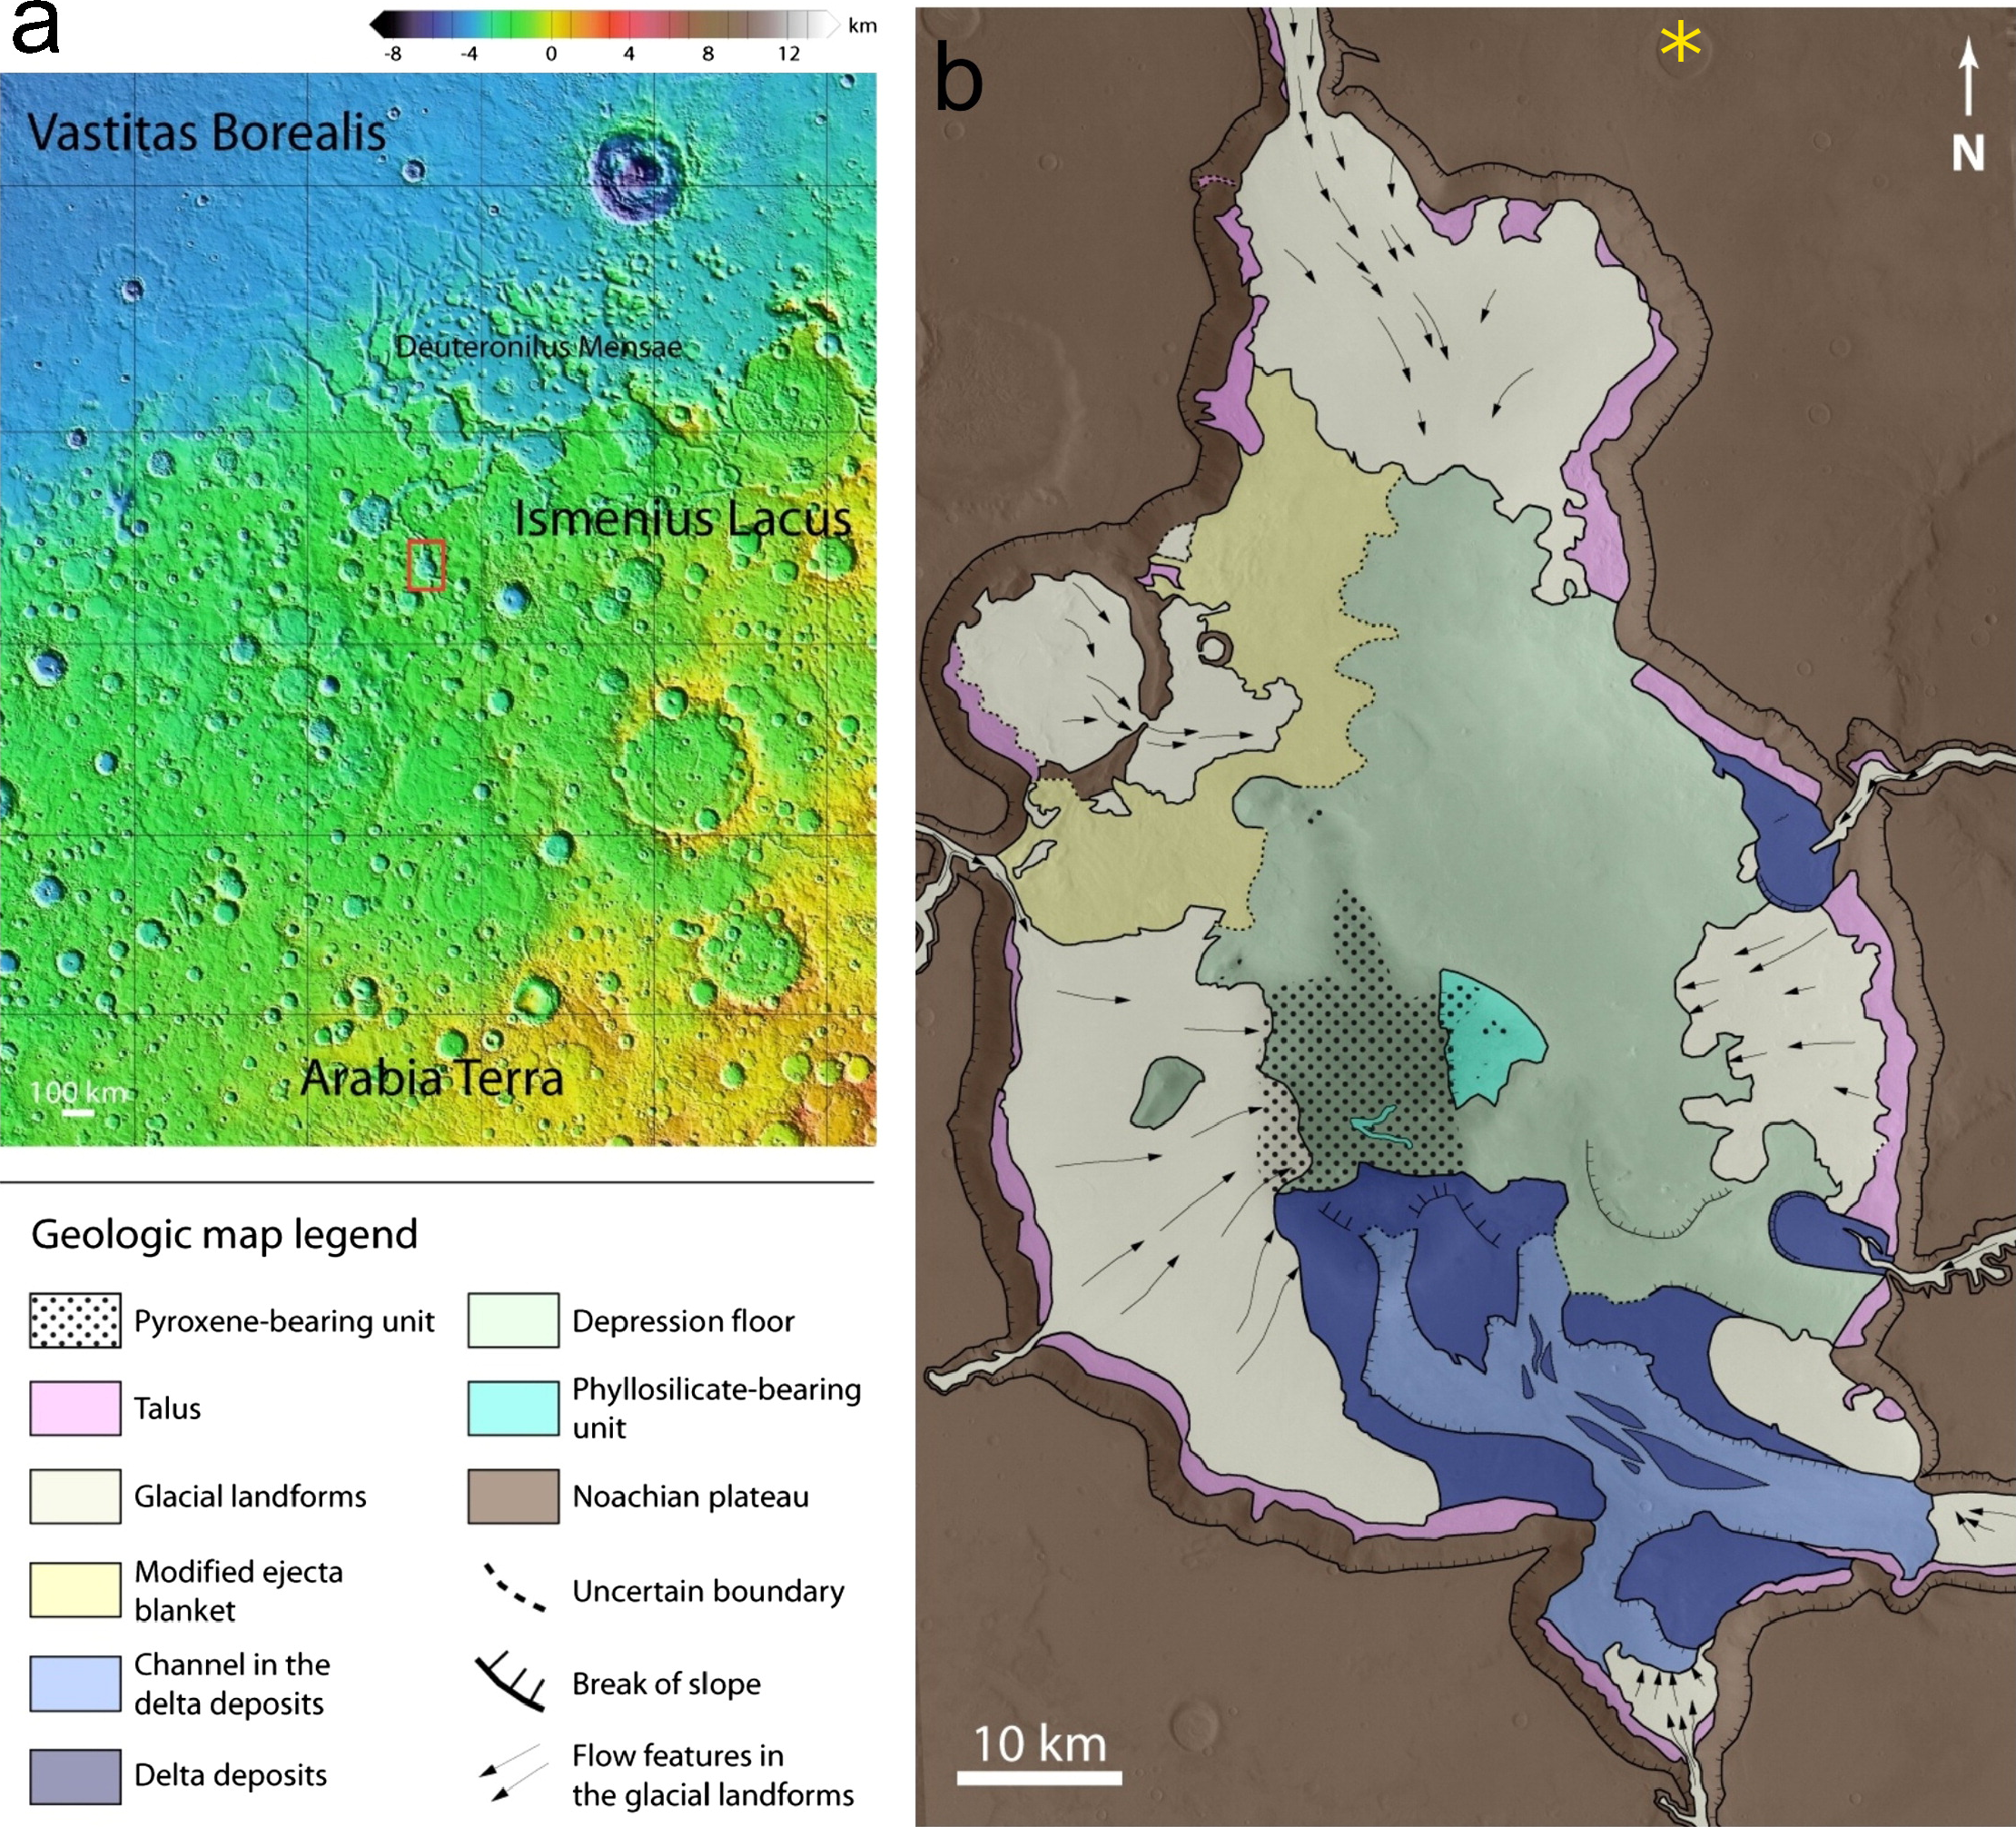
\includegraphics[width=0.6\linewidth]{sections/mars-solar-energy/mission-sites/images/ismenius-cavus.png}\\
  \caption[Geologic context of Ismenius Cavus mission site area]
          {Geologic context of Ismenius Cavus mission site area, taken from \citeother{Dehouck2010}. Location shown on a \ac{MOLA} reference map (a) and a geologic map of Ismenius Cavus (b). The yellow asterisk indicates the \ac{HiRISE} \ac{DTM} location which was used for mission scenario simulation.}
  \label{fig:mission-site-ismenius-cavus}
\end{figure}

% https://www.uahirise.org/dtm/dtm.php?ID=ESP_052945_2150

Supported science of interest are taken from \citeother{Dehouck2015}:
\begin{enumerate}[label=\textcolor{BulletBlue}{(\alph*)}]
    \item Potential for past habitability.
    \item Potential for organic matter with surface exposure.
    \item Noachian/Hesperian rocks with trapped atmospheric gases.
    \item High likelohood of surface-atmosphere exchange.
    \item Amazonian subsurface or high-latitude ice or sediment.
    \item Range of Martian geologic time; datable surfaces.
    \item Evidence of aqueous processes.
    \item Potential for interpreting relative ages.
    \item Near-surface ice, glacial or permafrost.
    \item Noachian or pre-Noachian bedrock units.
    \item Diversity of aeolian sediments and/or landforms.
\end{enumerate}

Supported resources of interest are also presented in \citeother{Dehouck2015} with clay minerals and water ice being two main resources for water. Furthermore, there is a potential for metal/silicon. These resources are located no more than \SI{3}{\meter} below the surface. Mobile material resources for construction purposes also exist.

\refFig{fig:sub:ismenius-cavus-dtm} shows a section of the \ac{DTM} which was loaded on the rover's mission simulation plaform. It features an exit breach in a well-preserved crater. The topography of the area is shown in \refFig{fig:sub:western-iani-chaos-dtm-altimetry}.
\vspace{0.5cm}

\begin{figure}[h]
\captionsetup[subfigure]{justification=centering}
\vspace{-2ex}
	\centering
    %% setup sizes
    \setlength{\subfigureWidth}{0.50\textwidth}
    \setlength{\graphicsHeight}{70mm}
    %% kill hyper-link highlighting
    \hypersetup{hidelinks=true}%
    %% the figures
    \begin{subfigure}[t]{\subfigureWidth}
        \centering
        \includegraphics[height=\graphicsHeight]{sections/mars-solar-energy/mission-sites/images/ismenius-cavus-dtm.png}
        \subcaption{\ac{DTM}}
        \label{fig:sub:ismenius-cavus-dtm}
    \end{subfigure}\hfill
    \begin{subfigure}[t]{\subfigureWidth}
        \centering
        \includegraphics[height=\graphicsHeight]{sections/mars-solar-energy/mission-sites/images/ismenius-cavus-dtm-altimetry.png}
  		\subcaption{Topography}
		\label{fig:sub:ismenius-cavus-dtm-altimetry}
	\end{subfigure}\\[0.8ex]
    \caption[Ismenius Cavus HiRISE digital terrain model]
            {Ismenius Cavus \ac{HiRISE} \ac{DTM}, taken from \citeother{AreoBrowser}. Image: \ac{NASA}/\ac{JPL}/University of Arizona.}
    \label{fig:ismenius-cavus}
\vspace{-2ex}
\end{figure}

\subsection{Daily Insolation}
Worst and best case daily insolations presented in this section are considered when sizing the rover's \ac{SA}. Optical depth is typically around $\tau = 0.4$ on clear days \citemarsenv{Smith2019} and $1 \leq \tau \leq 1.5$ during local dust storms \citemarsenv{Lemmon2015}. Daily insolations $\tau > 1.5$ were only considered for global dust storm season ($\SI{180}{\degree} < L_{s} < \SI{360}{\degree}$). Year long daily insolations for $\tau = 0.4$ at both sites are shown in \refFig{fig:plot:solar-insolations-for-different-beta} where the selected $\beta$ inclination angles are combined with their optimal $\gamma_c$ orientation angles. Descriptions of these angles are found in Appendix \ref{sec:Appendix:OptimalAngles}.

\begin{figure}[h]
\captionsetup[subfigure]{justification=centering}
\vspace{-2ex}
\centering
    %% setup sizes
    \setlength{\subfigureWidth}{0.50\textwidth}
    \setlength{\graphicsHeight}{60mm}
    %% kill hyper-link highlighting
    \hypersetup{hidelinks=true}%
    %% the figures
    \begin{subfigure}[t]{\subfigureWidth}
        \centering
            \includegraphics[height=\graphicsHeight]{sections/mars-solar-energy/mission-sites/plots/iani-chaos-solar-insolations-for-different-beta-inclinations.png}
            \subcaption{Iani Chaos.}
            \label{fig:plot:sub:solar-insolations-for-different-beta-iani-chaos}
    \end{subfigure}\hfill
    \begin{subfigure}[t]{\subfigureWidth}
        \centering
            \includegraphics[height=\graphicsHeight]{sections/mars-solar-energy/mission-sites/plots/ismenius-cavus-solar-insolations-for-different-beta-inclinations.png}
            \subcaption{Ismenius Cavus.}
            \label{fig:plot:sub:solar-insolations-for-different-beta-ismenius-cavus}
    \end{subfigure}\\[0.8ex]
    \caption[Daily insolations at mission sites]
    {Daily insolations at mission sites for different combinations of surface inclination and orientation angles.}
    \label{fig:plot:solar-insolations-for-different-beta}
\vspace{-2ex}
\end{figure}

Large values of $\beta$ are typically preferred in terms of resulting insolation. However, constraints imposed on the rover's active suspension system imposes a limit on the attainable inclination. As such, the optimal $\beta$ angle from which maximum insolation can be achieved, henceforth referred to as $\beta_{opt}$, may not be attainable. In such cases, the best possible $\beta$ angle is targetted, hereinafter referred to as $\beta_{best}$. Body pitch commands of up to \SI{10}{\degree} are experimentally evaluated during steep slope climbing in \citeother{Cordes2018}. Modeling higher pitch angles resulted in poor wheel-ground contact angle, as shown in \refFig{fig:postures-sa-beta}. This is due to the wheel-steering axis having the same tilt as the rover's body. The rover's attainable tilt is thus restricted to a maximum of \SI{10}{\degree}.

\begin{figure}[h]
\captionsetup[subfigure]{justification=centering}
%\vspace{-2ex}
	\centering
    %% setup sizes
    \setlength{\subfigureWidth}{0.50\textwidth}
    \setlength{\graphicsHeight}{50mm}
    %% kill hyper-link highlighting
    \hypersetup{hidelinks=true}%
    %% the figures
    \begin{subfigure}[t]{\subfigureWidth}
        \centering
        \includegraphics[height=\graphicsHeight]{sections/mars-solar-energy/mission-sites/images/sherpatt-render-surface-beta-13-deg.png}
        \subcaption{$\beta = \SI{13}{\degree}$}
        \label{fig:sub:postures-sa-beta-13-degree}
    \end{subfigure}\hfill
    \begin{subfigure}[t]{\subfigureWidth}
        \centering
        \includegraphics[height=\graphicsHeight]{sections/mars-solar-energy/mission-sites/images/sherpatt-render-surface-beta-22-deg.png}
  		\subcaption{$\beta = \SI{22}{\degree}$}
		\label{fig:sub:postures-sa-beta-22-degree}
	\end{subfigure}\\[0.8ex]
    \caption[SherpaTT body pitch \SI{13}{\degree} and \SI{22}{\degree}]
            {SherpaTT body pitch \SI{13}{\degree} and \SI{22}{\degree}.}
    \label{fig:postures-sa-beta}
\vspace{-2ex}
\end{figure}

\vspace{0.5cm}

Daily insolations on horizontal and inclined surfaces with $\beta_{best}=\pm\SI{10}{\degree}$\footnote{$\beta$ is positive in the northern hemisphere and negative in the southern hemisphere.} are presented in \refTab{tab:insolation-iani-chaos-clear-and-dusty-days} and \refTab{tab:insolation-iani-chaos-global-storm-days} for Iani Chaos and \refTab{tab:insolation-ismenius-cavus-clear-and-dusty-days} and \refTab{tab:insolation-ismenius-cavus-global-storm-days} for Ismenius Cavus. Gains obtained in daily insolation with an inclined surface are more pronounced for sites further away from the equator. For a typical optical depth of $\tau = 0.4$, the average daily insolation gain on the inclined surface is approximately \SI{7}{\percent} at Iani Chaos and \SI{9}{\percent} at Ismenius Cavus.
Due to the mostly diffuse composition of solar irradiance at higher optical depths, inclined surfaces become irrelevent during global dust storms. For $\tau \geq 2$, gains in daily insolation become negligeable at both mission sites.

\begin{table}[h]
\footnotesize
\centering
\caption[Worst and best case daily insolations for clear to dusty days at Iani Chaos]
{Worst and best case daily insolations for clear to dusty days at Iani Chaos. Daily insolation on an inclined surface $H_{\beta}$ is obtained with $\beta = \beta_{best} = \SI{-10}{\degree}$ and $\gamma_{c}$ set to optimal orientation angle.}
\label{tab:insolation-iani-chaos-clear-and-dusty-days}
\begin{tabular}{c|c|c|c|c|c|c|c|c|}
\cline{2-9}
\multicolumn{1}{l|}{} & \multicolumn{4}{c|}{\textbf{Worst Case}} & \multicolumn{4}{c|}{\textbf{Best Case}} \\ \hline
\multicolumn{1}{|c|}{$\tau$} & $L_{s}$ & $H_{h}$ & $H_{\beta}$ & $\%\:gain$ & $L_{s}$ & $H_{h}$ & $H_{\beta}$ & $\%\:gain$ \\ \hline
\multicolumn{1}{|c|}{\textbf{0.1}} & 80 & 3232 & 3721 & 15.13 & 221 & 5076 & 5695 & 12.19 \\ \hline
\multicolumn{1}{|c|}{\textbf{0.4}} & 81 & 2909 & 3166 & 8.85 & 218 & 4613 & 4933 & 6.93 \\ \hline
\multicolumn{1}{|c|}{\textbf{0.5}} & 81 & 2812 & 3025 & 7.58 & 218 & 4473 & 4736 & 5.89 \\ \hline
\multicolumn{1}{|c|}{\textbf{1.0}} & 82 & 2391 & 2479 & 3.67 & 214 & 3855 & 3959 & 2.69 \\ \hline
\multicolumn{1}{|c|}{\textbf{1.5}} & 82 & 2087 & 2125 & 1.81 & 213 & 3403 & 3444 & 1.19 \\ \hline
\end{tabular}
\end{table}


\vspace{0.5cm}

\begin{table}[h]
\footnotesize
\centering
\caption[Worst and best case daily insolations for global storm days at Iani Chaos]
{Worst and best case daily insolations for clear to global storm days at Iani Chaos. Daily insolation on an inclined surface $H_{\beta}$ is obtained with $\beta = \beta_{best} = \SI{-10}{\degree}$ and $\gamma_{c}$ set to optimal orientation angle.}
\label{tab:insolation-iani-chaos-global-storm-days}
\begin{tabular}{c|c|c|c|c|c|c|c|c|}
\cline{2-9}
\multicolumn{1}{l|}{} & \multicolumn{4}{c|}{\textbf{Worst Case}} & \multicolumn{4}{c|}{\textbf{Best Case}} \\ \hline
\multicolumn{1}{|c|}{$\tau$} & $L_{s}$ & $H_{h}$ & $H_{\beta}$ & $\%\:gain$ & $L_{s}$ & $H_{h}$ & $H_{\beta}$ & $\%\:gain$ \\ \hline
\multicolumn{1}{|c|}{\textbf{2.0}} & 360 & 2516 & 2519 & 0.10 & 212 & 3053 & 3066 & 0.42 \\ \hline
\multicolumn{1}{|c|}{\textbf{2.5}} & 360 & 2247 & 2243 & -0.18 & 211 & 2724 & 2723 & -0.02 \\ \hline
\multicolumn{1}{|c|}{\textbf{3.0}} & 360 & 1991 & 1985 & -0.32 & 210 & 2412 & 2406 & -0.27 \\ \hline
\multicolumn{1}{|c|}{\textbf{3.5}} & 360 & 1771 & 1763 & -0.45 & 210 & 2142 & 2134 & -0.37 \\ \hline
\multicolumn{1}{|c|}{\textbf{4.0}} & 360 & 1579 & 1572 & -0.44 & 209 & 1910 & 1901 & -0.47 \\ \hline
\multicolumn{1}{|c|}{\textbf{4.5}} & 360 & 1414 & 1406 & -0.54 & 209 & 1709 & 1700 & -0.54 \\ \hline
\multicolumn{1}{|c|}{\textbf{5.0}} & 360 & 1268 & 1261 & -0.58 & 209 & 1533 & 1523 & -0.62 \\ \hline
\end{tabular}
\end{table}


\vspace{0.5cm}

\begin{table}[h]
\footnotesize
\centering
\caption[Worst and best case daily insolations for clear to dusty days at Ismenius Cavus]
{Worst and best case daily insolations for clear to dusty days at Ismenius Cavus. Daily insolation on an inclined surface $H_{\beta}$ is obtained with $\beta = \beta_{best} = \SI{10}{\degree}$ and $\gamma_{c}$ set to optimal orientation angle.}
\label{tab:insolation-ismenius-cavus-clear-and-dusty-days}
\begin{tabular}{c|c|c|c|c|c|c|c|c|}
\cline{2-9}
\multicolumn{1}{l|}{} & \multicolumn{4}{c|}{\textbf{Worst Case}} & \multicolumn{4}{c|}{\textbf{Best Case}} \\ \hline
\multicolumn{1}{|c|}{$\tau$} & $L_{s}$ & $H_{h}$ & $H_{\beta}$ & $\%\:gain$ & $L_{s}$ & $H_{h}$ & $H_{\beta}$ & $\%\:gain$ \\ \hline
\multicolumn{1}{|c|}{\textbf{0.1}} & 274 & 2102 & 2762 & 31.42 & 127 & 4421 & 4925 & 11.40 \\ \hline
\multicolumn{1}{|c|}{\textbf{0.4}} & 273 & 1752 & 2030 & 15.85 & 125 & 4028 & 4289 & 6.49 \\ \hline
\multicolumn{1}{|c|}{\textbf{0.5}} & 273 & 1655 & 1869 & 12.93 & 124 & 3908 & 4122 & 5.48 \\ \hline
\multicolumn{1}{|c|}{\textbf{1.0}} & 273 & 1284 & 1345 & 4.75 & 121 & 3378 & 3461 & 2.44 \\ \hline
\multicolumn{1}{|c|}{\textbf{1.5}} & 273 & 1045 & 1061 & 1.57 & 120 & 2945 & 2973 & 0.96 \\ \hline
\end{tabular}
\end{table}


\vspace{0.5cm}

\begin{table}[h]
\footnotesize
\centering
\caption[Worst- and best-case daily insolations for global storm days at Ismenius Cavus]
{Worst- and best-case daily insolations for clear to global storm days at Ismenius Cavus. Daily insolation on an inclined surface $H_{\beta}$ is obtained with $\beta = \beta_{best} = \SI{10}{\degree}$ and $\gamma_{c}$ set to optimal orientation angle.}
\label{tab:insolation-ismenius-cavus-global-storm-days}
\begin{tabular}{c|c|c|c|c|c|c|c|c|}
\cline{2-9}
\multicolumn{1}{l|}{} & \multicolumn{4}{c|}{\textbf{Worst Case}} & \multicolumn{4}{c|}{\textbf{Best Case}} \\ \hline
\multicolumn{1}{|c|}{$\tau$} & $L_{s}$ & $H_{h}$ & $H_{\beta}$ & $\%\:gain$ & $L_{s}$ & $H_{h}$ & $H_{\beta}$ & $\%\:gain$ \\ \hline
\multicolumn{1}{|c|}{\textbf{2.0}} & 273 & 901 & 904 & 0.30 & 180 & 2155 & 2155 & 0.00 \\ \hline
\multicolumn{1}{|c|}{\textbf{2.5}} & 273 & 783 & 782 & -0.17 & 180 & 1899 & 1891 & -0.43 \\ \hline
\multicolumn{1}{|c|}{\textbf{3.0}} & 273 & 677 & 675 & -028 & 180 & 1664 & 1654 & -0.61 \\ \hline
\multicolumn{1}{|c|}{\textbf{3.5}} & 273 & 589 & 586 & -0.48 & 180 & 1467 & 1456 & -0.75 \\ \hline
\multicolumn{1}{|c|}{\textbf{4.0}} & 273 & 516 & 514 & -0.35 & 180 & 1300 & 1290 & -0.80 \\ \hline
\multicolumn{1}{|c|}{\textbf{4.5}} & 273 & 462 & 460 & -0.37 & 180 & 1158 & 1149 & -0.80 \\ \hline
\multicolumn{1}{|c|}{\textbf{5.0}} & 273 & 424 & 422 & -0.54 & 180 & 1038 & 1028 & -0.98 \\ \hline
\end{tabular}
\end{table}


The worst-case slope traverse is an on inclined surface facing opposite the equator. This can be mitigated by using the rover's suspension system to compensate with a tilt in the opposite direction, as illustrated in \refFig{fig:sub:rover-on-slope-beta} where $B$ denotes the slope surface inclination angle and $\beta$ the \ac{SA} surface inclination angle. This scenario will be further explored in \refSec{sec:Design:Simulation}. By way of example, at Ismenius Cavus for $\tau = 0.4$ and $L_{s}=\SI{270}{\degree}$, descending a \SI{30}{\degree} slope bearing North results in a daily insolation of \SI{319}{Whm^{-2}}. This can be increased to \SI{767}{Whm^{-2}} by decreasing $\beta$ from \SI{30}{\degree} to \SI{25}{\degree} after tilting the rover southwards by \SI{5}{\degree} so that $\beta < B$ with $\beta = \SI{25}{\degree}$. A \SI{10}{\degree} tilt would increase the daily insolation to \SI{1046}{Whm^{-2}} with $\beta = \SI{20}{\degree}$.


\begin{figure}[h]
\captionsetup[subfigure]{justification=centering}
%\vspace{-2ex}
	\centering
    %% setup sizes
    \setlength{\subfigureWidth}{0.50\textwidth}
    \setlength{\graphicsHeight}{40mm}
    %% kill hyper-link highlighting
    \hypersetup{hidelinks=true}%
    %% the figures
    \begin{subfigure}[t]{\subfigureWidth}
        \centering
        \includegraphics[height=\graphicsHeight]{sections/mars-solar-energy/mission-sites/images/stick-rover-beta-large.png}
        \subcaption{$\beta = B$}
        \label{fig:sub:rover-on-slope-beta-large}
    \end{subfigure}\hfill
    \begin{subfigure}[t]{\subfigureWidth}
        \centering
        \includegraphics[height=\graphicsHeight]{sections/mars-solar-energy/mission-sites/images/stick-rover-beta-small.png}
  		\subcaption{$\beta < B$}
		\label{fig:sub:rover-on-slope-beta-small}
	\end{subfigure}\\[0.8ex]
    \caption[Slope compensation with active suspension system]
            {Slope compensation with active suspension system to reduce the \ac{SA} surface inclination angle. Slope inclination angle $B = \SI{30}{\degree}$. In (a), $\beta = B = \SI{30}{\degree}$. In (b), the rover is tilted  \SI{10}{\degree} in the opposite direction of the slope so that $\beta = \SI{20}{\degree}$.}
    \label{fig:sub:rover-on-slope-beta}
%\vspace{-2ex}
\end{figure}


\subsection{Summary}
Available solar insolation have been constrained by identifying two mission sites based on set of selection criteria. The need to navigate complex topographic morphologies at these sites also introduces considerations for \ac{SA} inclination strategies. Large differences in planetary latitudes between both sites ensures that several environmental variations are considered.


\section{Summary and Conclusion}
\label{sec:MarsSolarEnergy:SummaryAndConclusion}
Understanding the dynamics of the Martian solar radiation environment is a crucial prequisite to  conceptualizing feasible mission scenarios. In this chapter, the potenial solar power and energy outputs were constrainted with mission site selections. Two locations were identified so that rover task planning and \ac{SA} sizing processes may appreciate a richer set of consequences tied to a wider range of environmental variables.
